\documentclass{article}


\usepackage[a4paper,top=1cm,bottom=1cm,left=1cm,right=1cm,marginparwidth=
1cm]{geometry}


\usepackage{multicol}
\PassOptionsToPackage{hyphens}{url}\usepackage{hyperref}

\usepackage{graphicx}
\usepackage[font=small,skip=4pt]{caption}
\graphicspath{ {.} }

\pagenumbering{gobble}

\title{The challenge of running Python on the Arduino}
\author{Christian Krause\\[0.1cm]{\small Supervisor: Helmut Ruf}}
\date{\small Student Research Center Baden-Württemberg Gearmany}

\usepackage{etoolbox}
\makeatletter
\patchcmd{\@maketitle}{\null\vskip 2em}{}{}{}
\makeatother

\begin{document}
\maketitle
\begin{multicols}{2}
\section{The Arduno Microcontroller}
The Arduino is a very popular microcontroller that is often used to teach the basics of programming at schools. The programming language used for the Arduino is almost always C, which is a compiled low-leval programming language. This means that it is very fast and uses a small amount of memory. The drawback is, that C is more difficult to learn than higher-level programming languages like Python. The difference between high- and low-level programming languages is the amount of control the user has over system. This can be a good thing for very performance critical applications, but high-level programming languages are generally easier.% For example in Python, it is very easy to create a List and to insert or remove values. When attempting this in C, you quickly encounter pointers and other low-level concepts that can be very difficult for beginners.

\section{Problem}
This raises the question why you wouldn't just use Python on the Arduino to teach programming. The Problem is, that the Arduino Uno only has 2 kb of Ram and 32 kb of program memory \cite{Q1}. The Python interpreter alone is over 30 mb big and it links into an even bigger standard libary. Running a Python executable requires a much faster CPU and orders of magnitude more RAM than the Arduino UNO has to offer. %So, at first glance, running Python on an Arduino seems impossible. But there is a project that attempts to solve this problem; MicroPython is an implementation of Python for microcontrollers, designed to use as few resources as possible. MicroPython is able to run a minimal subset of python with as little as 256 kb of flash and  16 kb of ram. But the Arduino Uno still only has an eigth of the capacity required to run MicroPython. 
The reason, why Python requires so much resources, is the way that it works different than C. To run a .c file, the C compiler translates it into machine code, which can then be executed. A python file on the other hand is run by the Python interpreter, which runs a python file line by line. This is a lot slower than a compiled C executable, but it enables a lot of the abstractions which make Python an easier, higher-level language than C.

\section{My solution: Pyduino}
My project, Pyduino aims to unify the easy syntax of Python with the speed of C to run Python-like programs on the Arduino Microcontroller. To achieve this, I developed a new programming language, Pyduino. The syntax of Pyduino is heavily inspired by Python \cite{Q2}. \\
%, with the only major difference being that the variables have a static type. This means that, in contrast to Python, you have to declare the type of a variable when you define it. The type of a variable can't be changed later in the program, so for example you can't assign a string to an integer variable, which is possible in Python. 
An important feature of Pyduino is, that the same code can run on the PC and the Arduino. This is very helpful, for example if you want to test a quick program, you can just run it on the PC without having to wait for the program to be uploaded to the Arduino, which can take several seconds. Running the same code on multiple platforms that are very different, like a PC and an Arduino comes with some challenges. For example printing output to a console is only possible on the PC, while the Arduino has the abiblity to use its IO pins to control LEDs or read from sensors. Pyduino solves this problem by utilizing the serial connection between the Arduino and the PC. If you program an Arduino conventionally using C, any output, that needs to be visible to the user is sent to the PC through this connection. In Pyudino programs, this bidirectional connection is not only used for output, but also for advanced features like function calls. If there is a program running on the PC that needs to use the IO pins of the Arduino, for example to turn on an LED or to read from a sensor, it sends a request to the Arduino using a serial protocol that I developed. The Arduino then executes this request and sends the result back to the PC. This connection can also be used for custom function calls between the Arduino and the PC. Whenever a function is defined in Pyduino, the programmer has the option to specify where it is executed. If for example the Arduino needs the result of a performance intensive function, you can add the @main decorator in front of the function, which tells Pyduino, that the function has to executed on the PC. Whenever the Arduino wants this function to be executed, it sends a request to the PC, which then executes the function and sends the result back to the Arduino.\\
In some cases, this can lead to massive performance imporvements. In this example, I used a recursive Fibonacci implementation to compute fib(40). If you run this function only on the Arduino, it takes about 18 minutes to complete. If the function is marked with the @main decorator to run on the PC, it takes about 440 ms to run it directly on the PC, calling it from the Arduino takes 447 ms. If you implement the fibonacci function in C and run it on the PC, it takes 436 ms to complete, while the Python implementation took 18 s. This shows that in some cases, Pyduino is almost as fast as C and much faster than Python. \\\\
\makebox[10pt][l]{%
\begin{minipage}{.5\textwidth}
\centering
    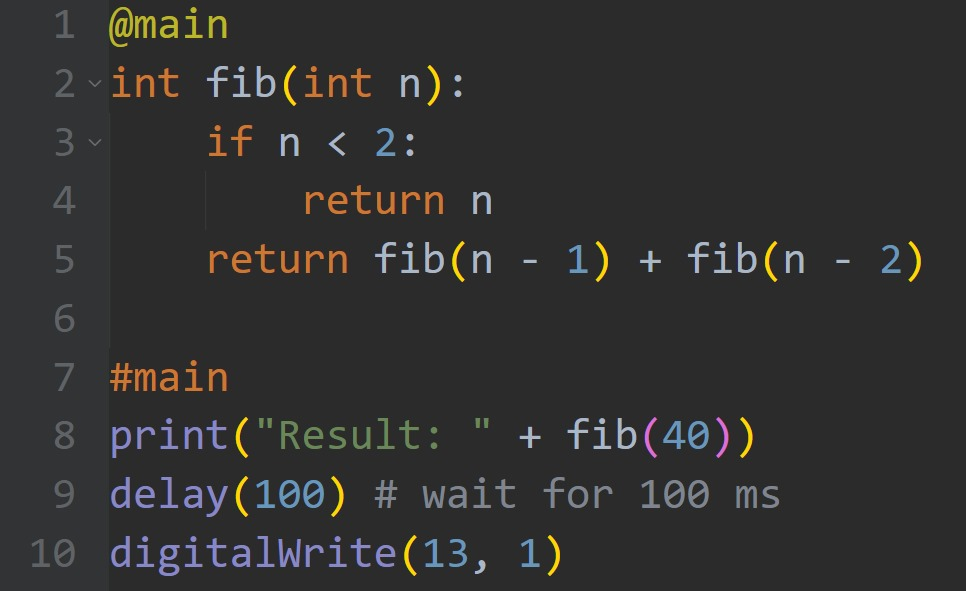
\includegraphics[width=7cm]{code}
 \captionof{figure}{Pyduino example code}
\end{minipage}
}
\\\\
Additionally, I developed a VS Code extension for Pyduino to make it as easy as possible to write Pyduino code \cite{Q3}. The extension can be easily installed from the VS Code marketplace and it provides syntax highlighting and error detection for Pyduino files. To run a Pyduino code, you just have to click the "Run Pyduino" Button and the extension takes care of compiling and running the code for the PC and the Arduino.
git


\begin{thebibliography}{99}
\bibitem{Q1} 
\url{https://docs.arduino.cc/hardware/uno-rev3/#tech-specs}
\bibitem{Q2}
\url{https://github.com/Bergschaf/Pyduino}
\bibitem{Q3}
\url{https://marketplace.visualstudio.com/items?itemName=Bergschaf.pyduino-extension}
\end{thebibliography}
\end{multicols}

\end{document}


